\section{Results} \label{sec:results}
% intro
Within this chapter, we present the crucial component of our study,
where we distill the essence of the extended PPI network by identifying the top 10 genes that stand out as significant contributors.
These genes have been selected based on their high connectivity and substantial change in gene activity within the network.\\

% General Result of the PageRank
Before exploring these key genes,
it is essential to provide an overview of the distribution of PageRank scores and $\Delta_{TPM}$ values across the gene dataset.
This will allow us to better understand the characteristics of our data and how they relate to one another.

The PageRank distribution exhibit an initial peak at a score of approximately 67,
which stands out as an outlier in comparison to other scores (see~\cref{fig:04_hist_pagerank}).
This peak is followed by a gradual decline to around 40, with subsequent scores showing progressively smaller differences
as they approach the mid-30s range.
Notably, once the scores fall to this level, the gaps between them become considerably narrower,
suggesting a pattern of logarithmic decay.
From the 1,033 relevant genes 155 have the lowest PageRank score of 0.151.
These genes consist of only one edge with a single protein that has not that many connections to other proteins.\\

\begin{figure}[h]
    \minipage{0.45\textwidth}
        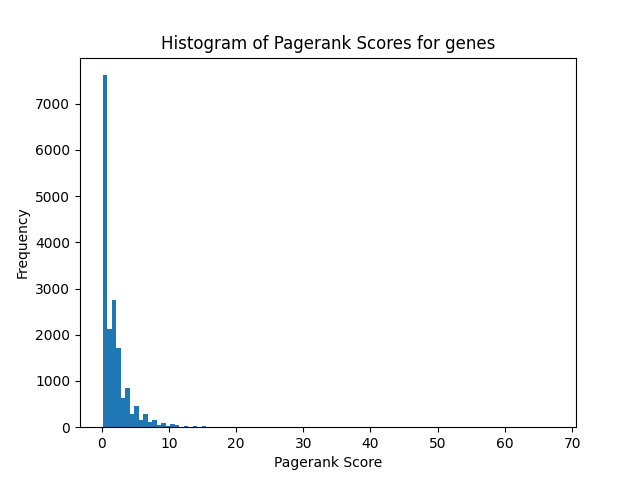
\includegraphics[width=\linewidth]{figures/04_hist_pagerank}
    \endminipage
    \hfill
    \minipage{0.45\textwidth}
      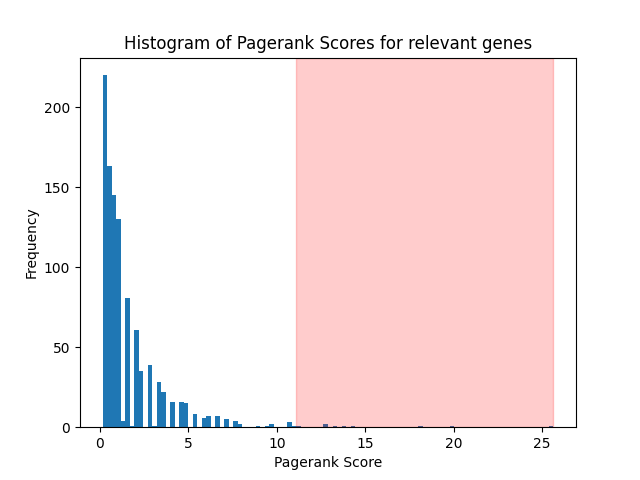
\includegraphics[width=\linewidth]{figures/04_hist_pagerank_relevant}
    \endminipage
    \caption{Comparison of the distribution of PageRank scores for all genes and genes with significant change in gene activity
    with highlighted area for the top 10 genes with the highest PageRank scores}
    \label{fig:04_hist_pagerank}
\end{figure}

The $\Delta_{TPM}$ values display a symmetric distribution with a pronounced peak around zero, showing a central tendency near the mean
(see~\cref{fig:04_delta_tpm_relevant}).
The data ranges from -0.709 to 0.423, showing moderate variability, and a normal-like distribution.
The significant change in gene activity is defined as a $\Delta_{TPM}$ value between -0.709 and -0.201 or 0.210 and 0.423.
We observe that 59\% of the relevant genes have an increase in gene activity and 41\% a decrease of activity.\\

\begin{figure}[!h]
    \centering
    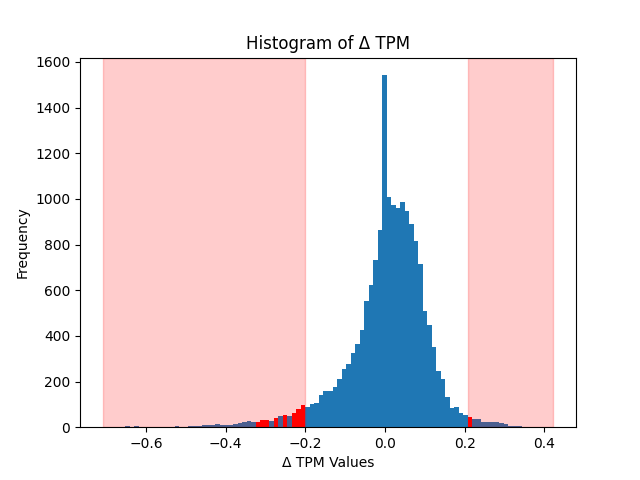
\includegraphics[height=\dfheightdouble]{figures/04_delta_tpm_relevant}
    \caption{Distribution of $\Delta_{TPM}$ values for genes with the area for significant change in gene activity highlighted in light red
    and the top 10 genes with the highest PageRank scores marked as red bars}
    \label{fig:04_delta_tpm_relevant}
\end{figure}


% Presentation of the 10 Genes
To identify the most significant genes, we choose to extract the \textbf{top 10 genes} with the highest PageRank scores from the list of relevant genes
as representative examples, as shown in \cref{fig:03_03_df_pagerank_relevant}.
These genes are not only highly connected within the network but also exhibit a substantial change in gene activity.
The PageRank scores are between 25.635 and 11.090,
while the $\Delta_{TPM}$ values span a range from 0.214719 to -0.317776, with only one gene showing a decrease in gene activity.\\


\begin{figure}[!h]
    \centering
    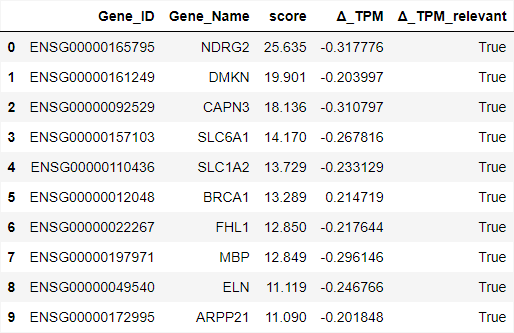
\includegraphics[height=\dfheightdouble]{figures/03_03_df_pagerank_relevant}
    \caption{Top 10 genes with the highest PageRank scores and a significant change in gene activity}
    \label{fig:03_03_df_pagerank_relevant}
\end{figure}

% One Example Gene
As an illustrative example of the structure of the top genes in our network,
we present a gene with high PageRank score and a significant change in gene activity
(see \cref{fig:04_example_gene}).\\

% Cypher: MATCH p = (g:gene {gene_name: 'ELN'})-[r]-(related) RETURN p
\begin{figure}[h]
    \centering
    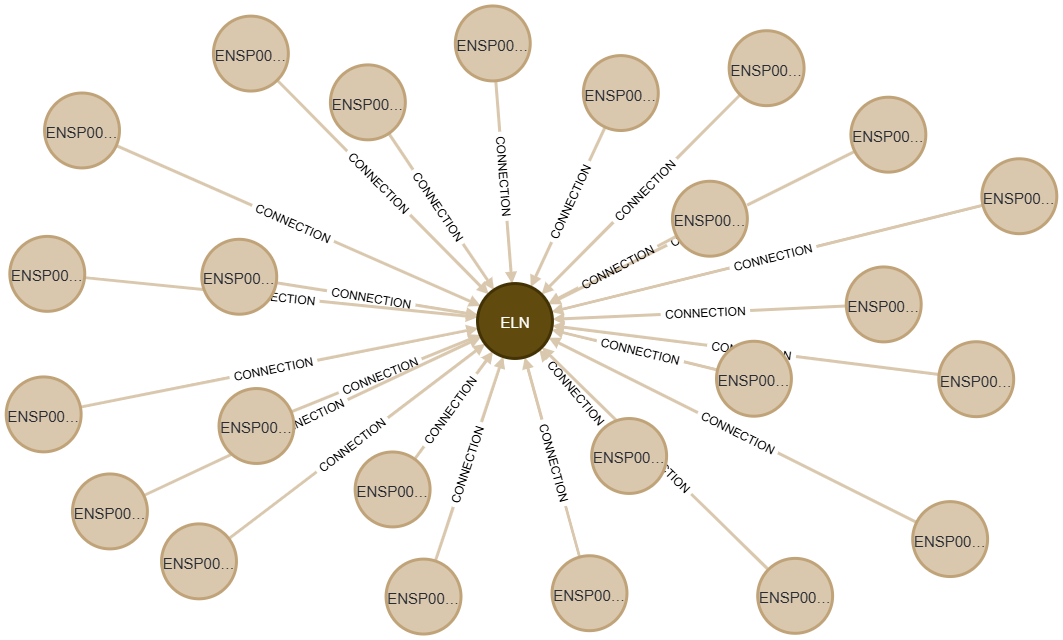
\includegraphics[height=\dfheightdouble]{figures/04_example_gene}
    \caption{An example extract from the graph database for a gene with high PageRank score and significant change in gene activity}
    \label{fig:04_example_gene}
\end{figure}

% Outro
The 10 genes presented here were identified as key players in the extended PPI network related to lung cancer.
By extracting these top-scoring genes, we not only highlight potential biomarkers but also
shed light on the intricate relationships within this complex biological system.
To further validate these findings, we will conduct a detailed analysis of the current literature and compare our results with existing studies.
